% Results section draft. Figures live in ../experiments/figs/ -- adjust
% \graphicspath if you move this file.
%
% Claims are graded by the evidence that supports them:
%   Sections 2-4 rest on pooled or high-decision-count data and are stated
%   plainly. Section 5 is a null. Section 6 is explicitly a hypothesis.
\documentclass[11pt]{article}

\usepackage[margin=1in]{geometry}
\usepackage{graphicx}
\usepackage{booktabs}
\usepackage{amsmath}
\usepackage{caption}
\usepackage[hidelinks]{hyperref}

\graphicspath{{../experiments/figs/}}
\captionsetup{font=small,labelfont=bf}

\title{Test-Time Search Degrades Control Policies When the Verifier Is Learned}
\author{Andrew Haggstrom}
\date{\today}

\begin{document}
\maketitle

\section{Experimental setup}

We evaluate test-time search on six Meta-World V3 manipulation tasks, selected
for long horizons (115--145 expert demonstration steps) and a spread of
difficulty. Long horizons matter: at an execution stride of $n_{\text{exec}}=8$
actions per replan, each episode presents 15--45 independent selection
decisions, so per-decision effects accumulate within an episode.

For each task we train a per-task behavior-cloning policy that predicts a
16-step action chunk from the 39-dimensional state, using 100 scripted-expert
demonstrations. Policies are deliberately trained to intermediate competence
(40--65\% success); a policy at ceiling leaves no room for search to help.
Candidate action chunks are drawn as Gaussian perturbations around the predicted
chunk.

\begin{table}[t]
\centering
\small
\begin{tabular}{lcccc}
\toprule
Task & Expert success & Demo length & Base policy & Decisions/episode \\
\midrule
peg-insert-side & 0.88 & 145 & 0.60 & $\sim$35 \\
basketball      & 0.91 & 132 & 0.45 & $\sim$40 \\
stick-pull      & 0.95 & 143 & 0.65 & $\sim$32 \\
shelf-place     & 0.96 & 114 & 0.65 & $\sim$31 \\
disassemble     & 0.98 & 135 & 0.65 & $\sim$31 \\
bin-picking     & 1.00 & 125 & 0.40 & $\sim$45 \\
\bottomrule
\end{tabular}
\caption{Task suite. Expert success is measured under the scripted policy used
for demonstration collection; base policy success is the cloned policy at $K=1$.}
\label{tab:tasks}
\end{table}

\paragraph{Selection arms.}
At each decision point the policy samples $K$ candidate chunks and one is
executed. We compare: \textbf{no search} ($K=1$); \textbf{random}, which selects
uniformly and controls for candidate count alone; \textbf{oracle}, which scores
each candidate by branching the true simulator; \textbf{learned dynamics}, which
scores by rolling a learned probabilistic ensemble forward four steps with a
learned value function bootstrapping the tail; \textbf{value best-of-$N$}; and
\textbf{self-consistency}, which selects the medoid of the candidate set and
uses no learned scorer at all. We sweep $K \in \{1,\dots,64\}$ over 50 episodes
per cell, nested so that all $K$ share a candidate pool, and paired across arms
by episode seed.

\paragraph{Exact simulator branching.}
The oracle arm requires that scoring a candidate leave no trace on the trunk
trajectory. We save and restore MuJoCo state using the
\texttt{mjSTATE\_INTEGRATION} specification rather than
\texttt{mjSTATE\_FULLPHYSICS}: the latter omits \texttt{qacc\_warmstart}, the
constraint solver's cached initial guess, and a differing warmstart causes the
solver to converge along a slightly different path. We additionally reapply the
warmstart after \texttt{mj\_forward}, which overwrites it as a side effect, and
we roll back mutable Python state on every wrapper in the environment chain, not
only the innermost environment. Without these, branching silently perturbs the
trajectory it branches from.

\section{Search succeeds given a perfect model}

Given true dynamics, additional candidates translate into better outcomes on
three of six tasks: basketball ($0.62 \to 0.92$), shelf-place
($0.66 \to 0.90$), and stick-pull ($0.50 \to 0.78$). A fourth, bin-picking,
improves marginally within noise. This establishes that the candidate sets
contain actions materially better than the policy's first sample, and that the
search procedure can find them. Without this control, later negative results
would be ambiguous between an ineffective search procedure and an inadequate
verifier.

\begin{figure}[t]
\centering
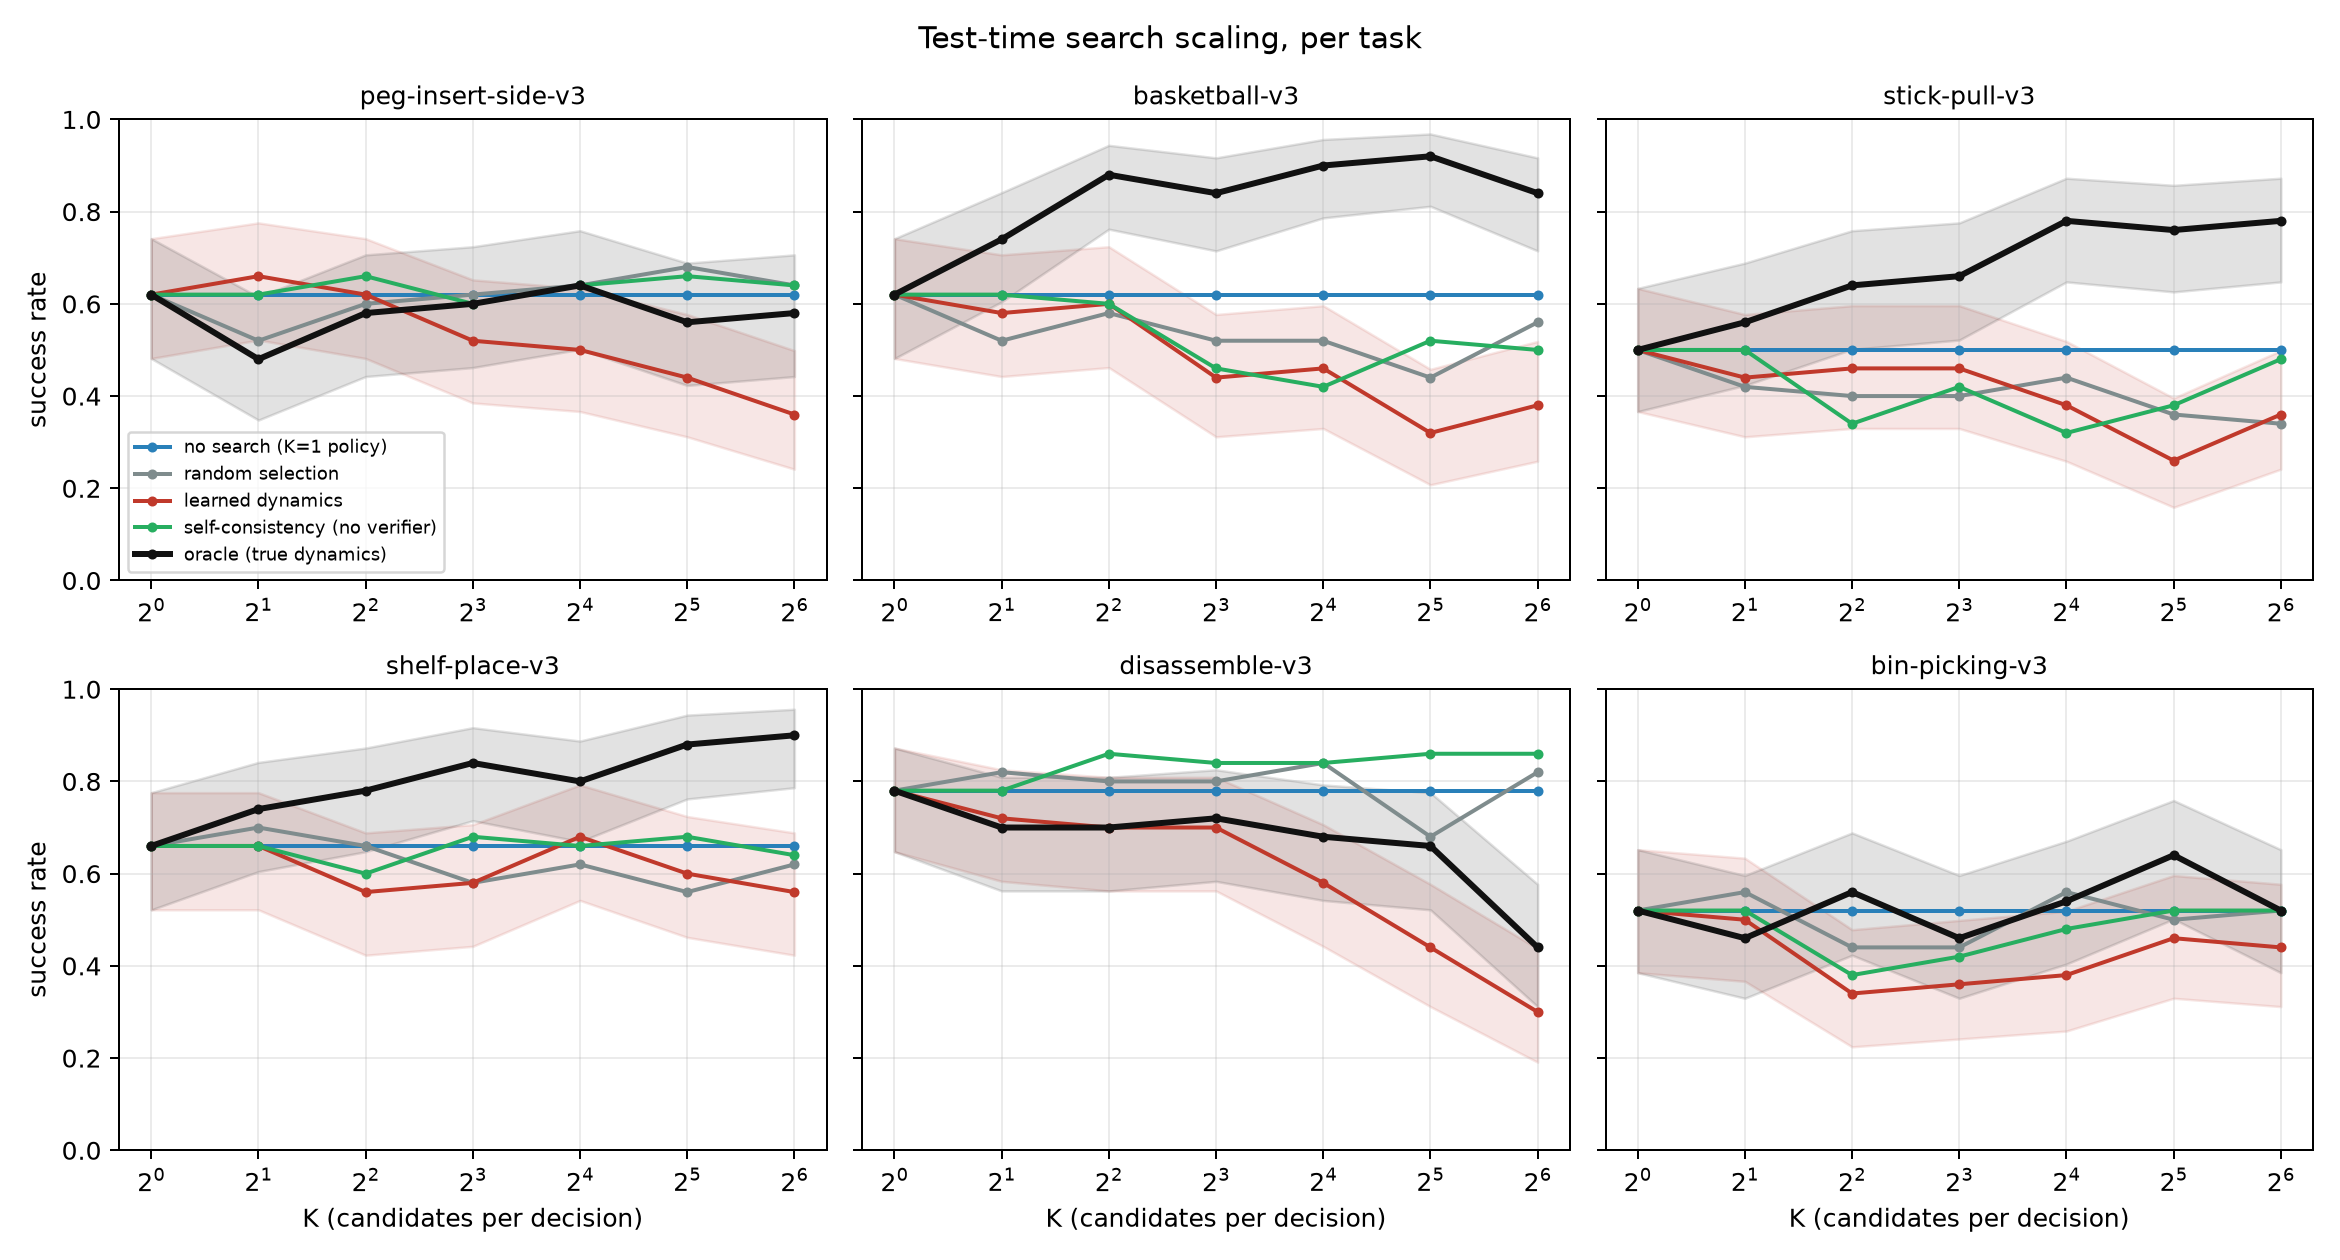
\includegraphics[width=\textwidth]{fig1_per_task.png}
\caption{Success rate versus candidate count $K$, per task, 50 episodes per
cell. The oracle arm (black) rises clearly on basketball, stick-pull, and
shelf-place. Per-task confidence bands overlap substantially at this sample
size; the pooled analysis in Figure~\ref{fig:pooled} carries the inference.
Note that the oracle \emph{declines} on disassemble, which we return to in
Section~\ref{sec:objective}.}
\label{fig:pertask}
\end{figure}

\section{With a learned verifier, search is worse than not searching}

Our central result is that selecting candidates by a learned verifier degrades
performance monotonically in $K$, and ends below random selection. Pooled across
all six tasks, success falls from $0.62$ at $K=1$ to $0.40$ at $K=64$, while
random selection remains near $0.58$ and the no-search baseline is flat at
$0.62$ by construction.

\begin{figure}[t]
\centering
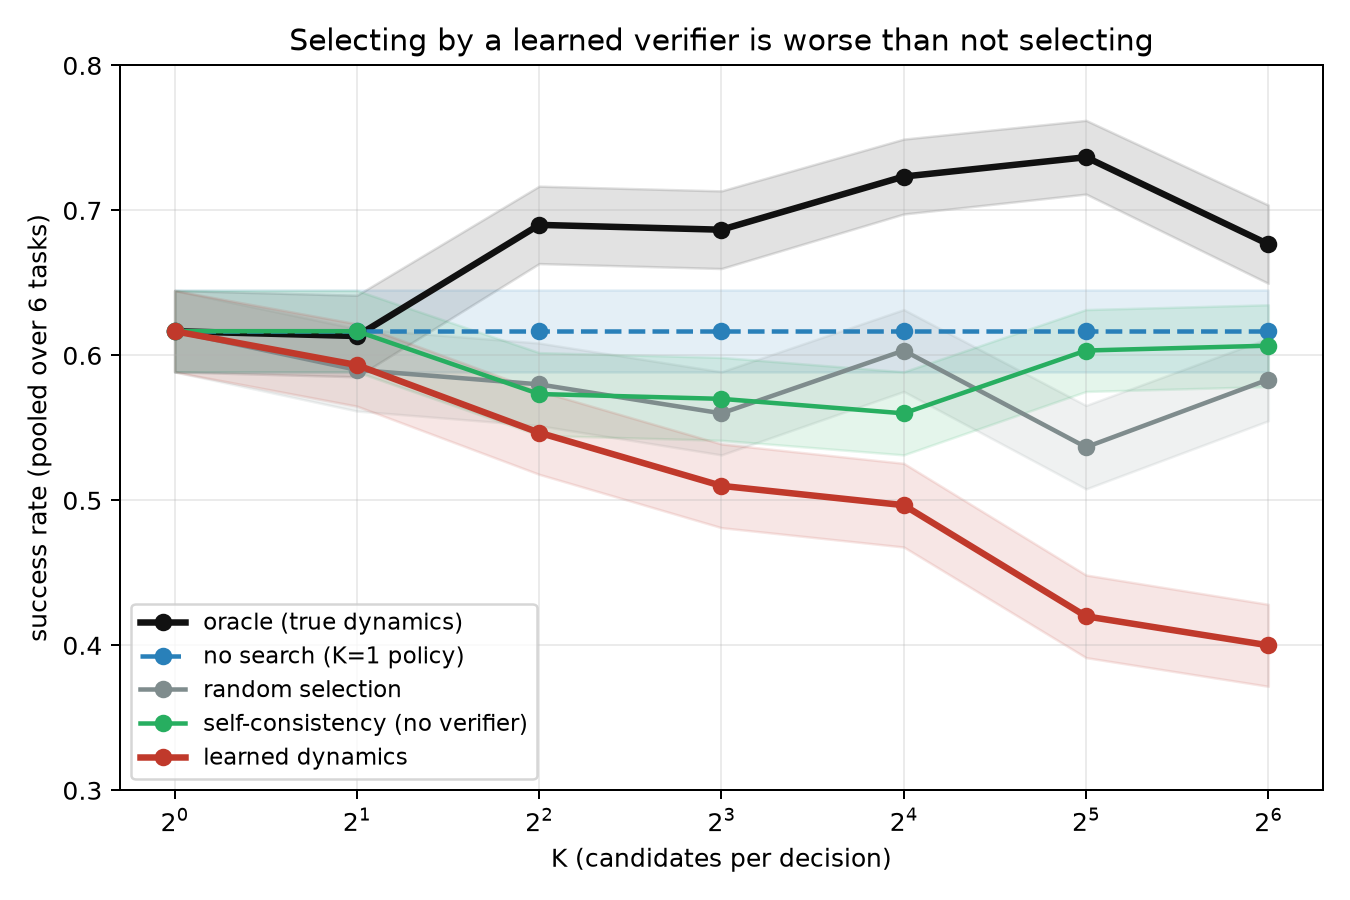
\includegraphics[width=0.85\textwidth]{fig2_pooled.png}
\caption{Success rate versus $K$, pooled over six tasks (300 episodes per cell,
shaded bands are $\pm1$ standard error). Selecting by the learned verifier
(red) falls well below both no-search (blue) and random selection (grey), while
the oracle (black) rises. The random control rules out candidate count as the
cause: the harm comes specifically from selecting on predicted value.}
\label{fig:pooled}
\end{figure}

Two features deserve emphasis. First, the random-selection control separates
``more candidates is harmful'' from ``choosing by predicted value is harmful''
and supports only the latter. Second, there is no rising phase: degradation
begins at $K=2$ and continues monotonically. This differs from reward-model
over-optimization in language models, where performance typically improves
before turning over.

Recent work on test-time scaling for robot policies reports gains rather than
degradation. Those evaluations generally use $K \le 32$ and shorter effective
horizons. We note below that per-decision harm in our setting is small
($\sim$5\%) and accumulates over 15--45 decisions per episode, which offers a
plausible reconciliation, though we do not test it directly.

\section{The verifier, not the search, is what fails}

To separate ``no better candidates exist'' from ``the verifier cannot identify
them,'' we audit selection directly. At each decision point we score the same
candidate pool two ways---with the learned verifier and with true simulator
rollouts---and record the true value of the candidate the learned verifier
chose, of the best candidate, and of the average candidate.

\begin{figure}[t]
\centering
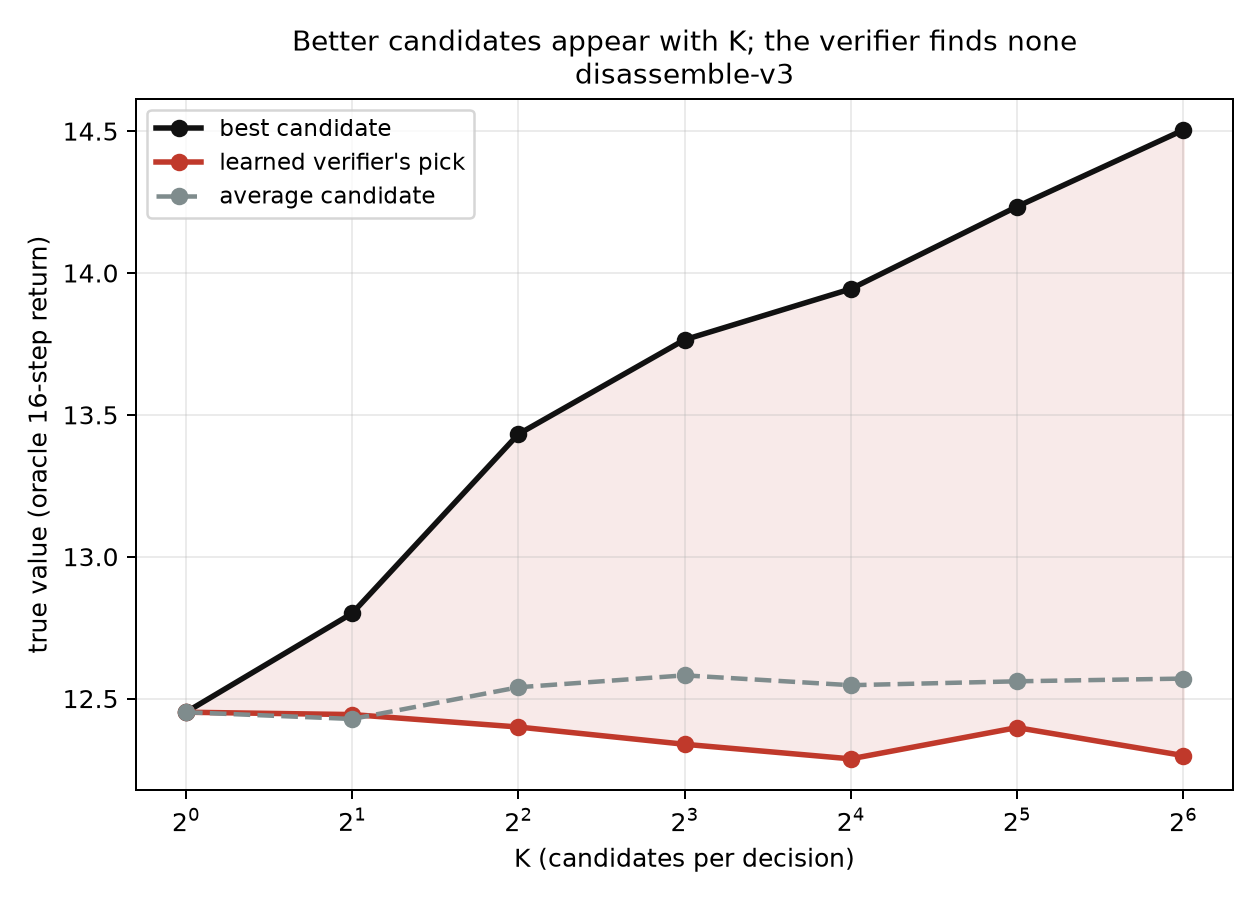
\includegraphics[width=0.8\textwidth]{fig3_audit.png}
\caption{Selection audit on disassemble, 435 decision points. As $K$ grows the
best available candidate improves substantially ($12.45 \to 14.50$ in true 16-step return), while the learned verifier's pick remains flat at $\sim$12.3,
statistically indistinguishable from the average candidate ($\sim$12.5).
Normalized regret is $0.93$--$1.08$ at every $K$.}
\label{fig:audit}
\end{figure}

Normalized regret, $(\text{best}-\text{picked})/(\text{best}-\text{mean})$, sits
at approximately $1.0$ across the full range of $K$: the learned verifier's
selection is worth no more than an arbitrary candidate. Better candidates
demonstrably appear as $K$ grows, and the verifier finds none of them.

One tension remains unresolved. Regret near $1.0$ implies picks that are average
\emph{with respect to true short-horizon return}, yet the learned arm's task
success (0.30) falls far below random selection's (0.82) on this task. The
learned verifier therefore appears to select on some feature that is
uncorrelated with short-horizon return while being harmful to eventual task
completion. We do not identify that feature.

We also note that the per-decision effect is small---roughly a 5\% reduction in
success probability relative to an average candidate---while the episode-level
effect is a 48-point drop. The mechanism is accumulation across many decisions,
not any single catastrophic choice.

\section{Uncertainty penalties do not help}

A natural remedy is to penalize candidates the model is uncertain about. We add
$-\beta \cdot d$ to each candidate's score, where $d$ is ensemble disagreement,
and sweep four values of $\beta$ per task. Values are calibrated per task
against the measured ratio of return spread to disagreement spread at real
decision points; naive values chosen without calibration would have been
20--400$\times$ too small to have any effect.

\begin{table}[t]
\centering
\small
\begin{tabular}{lccccccc}
\toprule
$\beta$ rank & $K{=}1$ & $K{=}2$ & $K{=}4$ & $K{=}8$ & $K{=}16$ & $K{=}32$ & $K{=}64$ \\
\midrule
0 (none)     & 0.62 & 0.59 & 0.55 & 0.51 & 0.50 & 0.42 & 0.40 \\
1            & 0.62 & 0.60 & 0.54 & 0.52 & 0.49 & 0.41 & 0.41 \\
2            & 0.62 & 0.61 & 0.58 & 0.54 & 0.48 & 0.41 & 0.43 \\
3 (largest)  & 0.62 & 0.60 & 0.59 & 0.53 & 0.49 & 0.44 & 0.41 \\
\bottomrule
\end{tabular}
\caption{Pooled success by disagreement-penalty strength. Curves are
indistinguishable across two orders of magnitude in $\beta$.}
\label{tab:beta}
\end{table}

Degradation is essentially unchanged across two orders of magnitude in $\beta$.
Ensemble disagreement, at least as computed here, does not identify the
candidates that search should avoid.

\section{Model quality: a null result}

We further asked whether degradation scales with dynamics-model error. We
trained model ladders spanning a 12$\times$ range in median 4-step prediction
error (0.19--2.22$\sigma$ on disassemble; 0.11--4.44$\sigma$ on basketball) by
jointly reducing training data, network width, and training length, and reran
the sweep at each rung. We observed no systematic relationship between model
error and degradation. With four rungs per task and a per-condition standard
error near 0.07, this experiment cannot distinguish a modest relationship from
none, and we report it as a null rather than as evidence of independence.

\section{What survives: verifier-free selection}

Self-consistency---selecting the candidate closest to all others, using no
learned scorer---does not degrade. Pooled success is $0.62$ at $K=1$ and $0.61$
at $K=64$; on disassemble it improves ($0.78 \to 0.86$). Having no learned
proxy, it has no proxy to over-optimize. It is also the cheapest arm, requiring
no additional model. Where a verifier of uncertain quality is the only option,
this is the safer default.

\section{A distinct failure mode: objective misspecification}
\label{sec:objective}

On disassemble the oracle arm also degrades ($0.78 \to 0.44$) despite having
perfect dynamics, which implicates the scoring objective rather than model
error. Three observations are consistent with this: the oracle declines; a
success-based audit finds that the highest 16-step-return candidate succeeds no
more often than an average one; and model quality across a 12$\times$ range
produces no trend.

\begin{figure}[t]
\centering
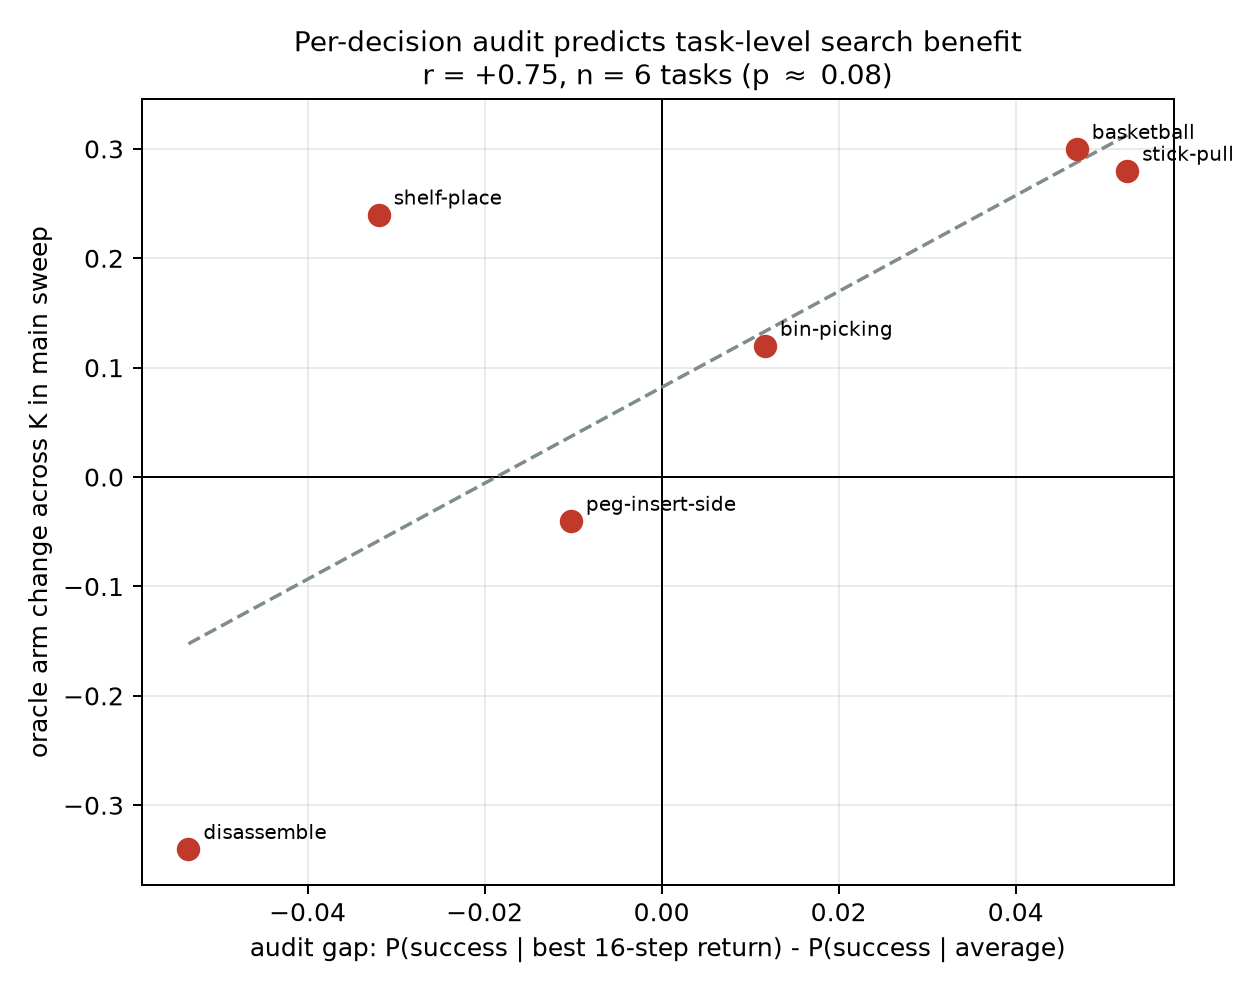
\includegraphics[width=0.7\textwidth]{fig6_audit_scatter.png}
\caption{Per-task audit gap---the success advantage of the highest-16-step-return
candidate over an average candidate---against the change in oracle-arm success
across $K$ in the main sweep. One point per task, $r=+0.75$, $n=6$
($p \approx 0.08$). Shelf-place is discordant.}
\label{fig:scatter}
\end{figure}

The relationship in Figure~\ref{fig:scatter} is suggestive but not established:
$n=6$ tasks, individual audit gaps are within noise at 90 decision points each,
and shelf-place has a negative gap despite a strongly positive oracle slope. We
present this as a hypothesis the data is consistent with---that maximizing
short-horizon return is misaligned with task completion on some tasks, and that
search amplifies this misalignment regardless of model quality---rather than as
a finding.

\section{Limitations}

\begin{itemize}
\item \textbf{One policy class.} Candidates are Gaussian perturbations of a
single predicted action chunk rather than samples from a multimodal
distribution. Candidate diversity is a plausible moderator we did not vary; a
diffusion policy might behave differently.
\item \textbf{Single seed.} One policy, dynamics model, and value function per
task. We have no estimate of training variance.
\item \textbf{Statistical power.} 50 episodes per cell gives a standard error
near 0.07. This is adequate for the 22-point main effect but marginal for every
secondary comparison, and per-task curves should be read as context rather than
as independent evidence.
\item \textbf{The oracle is not an upper bound.} It has perfect dynamics but an
imperfect objective, and Section~\ref{sec:objective} shows this matters.
\item \textbf{Simulation and state observations only.} No pixel observations, no
physical robot.
\end{itemize}

\end{document}
